\documentclass[12pt,runningheads]{article}
\usepackage[utf8]{inputenc}
\usepackage{float}

%enable apa
\usepackage[english]{babel}
\usepackage{csquotes}

%some additional packages
\usepackage[pdftex]{graphicx}

\begin{document}

\title{Parflow Performance Benchmark API Documentation}
\author{Nicholas Prussen}
\maketitle
\newpage

\tableofcontents

\newpage

\section{Introduction}
This documentation provides information on the request type of each API endpoint as well as the format of the data returned and/or received. These endpoints will be split into three groups (Adapt/Princeton/General), as certain endpoints are used exclusively on the different react apps.


\section{Adapt Endpoints}

\subsection{getHostnames}
Request Type: \textbf{GET}
\newline
Request Address: \textbf{/gethostnames}
\newline

This endpoint takes in no data and will return a list of all \textbf{unique} hostnames found among the "run\_information" document embedded in the top level MongoDB documents.

It should be noted that only the documents uploaded using the Adapt uploader script found in ParFlow Performance Testing will have the "run\_information" embedded document field, so this will not return any document information taken from data uploaded using Shweta's uploader script.

\subsubsection{Data Format}
\textbf{Required Data}: \textbf{N/A}
\newline
\newline
\textbf{Returned Data}:
\newline
\newline
This endpoint will return a JSON document with a key/value containing a list of unique hostnames found in the database. An example of what this JSON document looks like can be found in Figure \ref{fig:getHostnames}.

\begin{figure}[H]
    \centering
    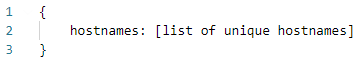
\includegraphics{img/gethostnames.PNG}
    \caption{getHostnames Returned Data Format}
    \label{fig:getHostnames}
\end{figure}


\subsection{getDomainsByHostname}
Request Type: \textbf{POST}
\newline
Request Address: \textbf{/getdomainsbyhostname}
\newline

This endpoint takes in a JSON document containing a defined hostname with which to query all existing documents that contain this hostname in their "run\_information" field, if it exists. The returned data will also be a JSON document that contains all \textbf{unique} domain names found from documents containing the hostname.

It should be noted that only the documents uploaded using the Adapt uploader script found in ParFlow Performance Testing will have the "run\_information" embedded document field, so this will not return any document information taken from data uploaded using Shweta's uploader script.

\subsubsection{Data Format}
\textbf{Required Data}:
\newline
\newline
This endpoint takes in a JSON document in the request body using the format found in Figure \ref{fig:getdomainsbyhostname}. The "String" field should be replaced with the hostname being used to query.
\begin{figure}[h!]
    \centering
    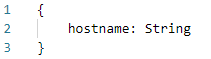
\includegraphics{img/getdomainsbyhostname.PNG}
    \caption{getDomainsByHostname Received Data Format}
    \label{fig:getdomainsbyhostname}
\end{figure}
\newline
\textbf{Returned Data}:
\newline
\newline
This endpoint will return a JSON document with a list containing all unique domains found in the database under the hostname provided. An example of what this JSON document looks like can be found in Figure \ref{fig:getdomainsbyhostname2}.

\begin{figure}[H]
    \centering
    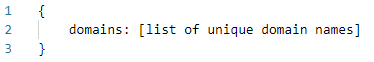
\includegraphics{img/getdomainsbyhostname2.PNG}
    \caption{getDomainsByHostname Returned Data Format}
    \label{fig:getdomainsbyhostname2}
\end{figure}



\subsection{getDocumentsByHostnameDomain}
Request Type: \textbf{POST}
\newline
Request Address: \textbf{/getdocumentsbyhostnamedomain}
\newline

This endpoint takes in a JSON document containing a defined hostname and domain with which to query all existing documents that contain the defined hostname and domain in their "run\_information" field, if it exists. The returned data will also be a JSON document that contains all \textbf{unique} documents found in the database, but separated into different documents based on core counts.

It should be noted that only the documents uploaded using the Adapt uploader script found in ParFlow Performance Testing will have the "run\_information" embedded document field, so this will not return any document information taken from data uploaded using Shweta's uploader script.

\subsubsection{Data Format}
\textbf{Required Data}:
\newline
\newline
This endpoint takes in a JSON document in the request body using the format found in Figure \ref{fig:getdocumentsbyhostnamedomain1}. The "String" fields should be replaced with the hostname and domain being used to query. It should be noted that "runname" was the previous key used to define the domain used and the "String" field following "runname" should be the domain.
\begin{figure}[H]
    \centering
    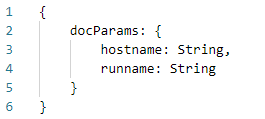
\includegraphics{img/getdocumentsbyhostnamedomain1.PNG}
    \caption{getDocumentsByHostnameDomain Received Data Format}
    \label{fig:getdocumentsbyhostnamedomain1}
\end{figure}
\textbf{Returned Data}:
\newline
\newline
This endpoint will return a JSON document that contains all unique MongoDB documents queried by the hostname and domain, but will split them up based on their core count to ease use in the react app. The API will generate keys in the top level document based off all unique core counts found among the documents. These keys will each have a value containing an embedded document that will hold all MongoDB documents that have a core count matching those keys. These documents are labeled using their provided MongoDB \_id as a key and the value being the raw document data. An example of what this JSON document looks like can be found in Figure \ref{fig:getdocumentsbyhostnamedomain2}.

\begin{figure}[H]
    \centering
    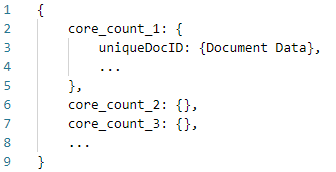
\includegraphics{img/getdocumentsbyhostnamedomain2.PNG}
    \caption{getDocumentsByHostnameDomain Returned Data Format}
    \label{fig:getdocumentsbyhostnamedomain2}
\end{figure}



\section{Princeton Endpoints}

\subsection{getDocumentsPrinceton}
Request Type: \textbf{POST}
\newline
Request Address: \textbf{/getdocumentsprinceton}
\newline

This endpoint takes in a JSON document containing a defined number of days to query documents by into the past. The returned data will also be a JSON document that contains all \textbf{unique} documents found in the database that were uploaded inside the window of the provided amount of days.

It should be noted that this endpoint specifically checks for the existence of the "globalid" field to include only documents created by Shweta's uploader script. This will exclude all documents uploaded by the Adapt uploader script as it does not insert the "globalid" field when uploading.

\subsubsection{Data Format}
\textbf{Required Data}:
\newline
\newline
This endpoint takes in a JSON document in the request body using the format found in Figure \ref{fig:getdocumentsprinceton1}. The "Integer" field should be replaced with the number of days being used to query back to.
\begin{figure}[H]
    \centering
    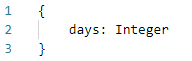
\includegraphics{img/getdocumentsprinceton1.PNG}
    \caption{getDocumentsPrinceton Received Data Format}
    \label{fig:getdocumentsprinceton1}
\end{figure}
\textbf{Returned Data}:
\newline
\newline
This endpoint will return a JSON document with a list that contains all unique MongoDB documents that were found within the amount of days provided in the POST request body. An example of what this JSON document looks like can be found in Figure \ref{fig:getdocumentsprinceton2}.

\begin{figure}[H]
    \centering
    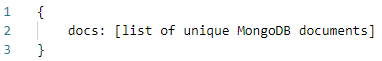
\includegraphics{img/getdocumentsprinceton2.PNG}
    \caption{getDocumentsPrinceton Returned Data Format}
    \label{fig:getdocumentsprinceton2}
\end{figure}


\section{Generic Endpoints}

\subsection{getDocumentByID}
Request Type: \textbf{POST}
\newline
Request Address: \textbf{/getdocumentbyid}
\newline

This endpoint takes in a JSON document containing a defined document ID to return the raw data of the document found inside the database. This endpoint will also return a JSON document containing an error if the provided ID was either of invalid format, or was not found inside the database.

It should be noted that this endpoint will find any documents in the database regardless of who uploaded it as it queries based off the Mongo provided \_id which all documents have.

\subsubsection{Data Format}
\textbf{Required Data}:
\newline
\newline
This endpoint takes in a JSON document in the request body using the format found in Figure \ref{fig:getdocumentbyid1}. The "String" field should be replaced with the ID being used to query.
\begin{figure}[H]
    \centering
    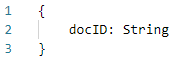
\includegraphics{img/getdocumentbyid1.PNG}
    \caption{getDocumentByID Received Data Format}
    \label{fig:getdocumentbyid1}
\end{figure}
\textbf{Returned Data}:
\newline
\newline
This endpoint will return two possible JSON documents depending on the success of the query. To avoid errors, the API will check if the ID provided is both a valid ObjectID and if the query actually returned some document data. If neither of those checks pass, the API will return a JSON document in the format found in Figure \ref{fig:getdocumentbyid3}.
\begin{figure}[H]
    \centering
    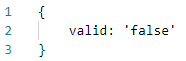
\includegraphics{img/getdocumentbyid3.PNG}
    \caption{getDocumentByID Returned Data Format}
    \label{fig:getdocumentbyid3}
\end{figure}
Otherwise, a successful query will return a variable JSON document that holds only the raw document data found by the query. This is essentially plucking a document out of the database without any modifications to it's structure An example of what this JSON document looks like can be found in Figure \ref{fig:getdocumentbyid2}.

\begin{figure}[H]
    \centering
    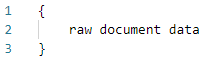
\includegraphics{img/getdocumentbyid2.PNG}
    \caption{getDocumentByID Returned Data Format}
    \label{fig:getdocumentbyid2}
\end{figure}



\newpage

\end{document}
